\begin{figure*}[t]
\centering
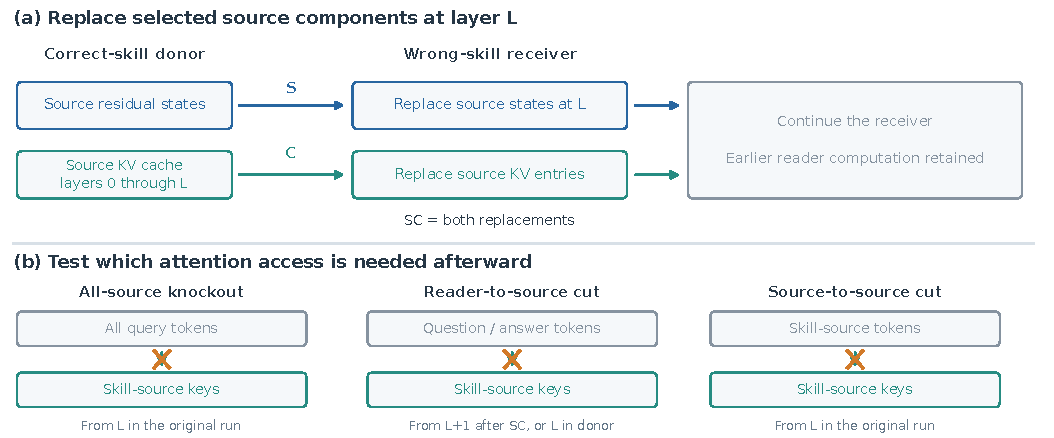
\includegraphics[width=\textwidth]{fig-intervention-design.pdf}
\caption{Intervention design. (a) The correct-skill donor supplies source
residual states ($S$), source-position key/value (KV) entries through layer $L$ ($C$),
or both ($SC$) to the wrong-skill receiver. Earlier reader computation
is retained. (b) Attention cuts distinguish access by reader tokens
from updates within the skill source. After $SC$, the reader cut begins
at $L+1$. In the original correct-skill run, path cuts begin at $L$.
All cuts continue through the remaining prompt processing and decoding.}
\Description{A component-level diagram shows donor source states and caches
replacing selected receiver components while earlier reader computation is
retained. Three attention paths illustrate cumulative knockout, reader cuts
and source-self cuts.}
\label{fig:design}
\end{figure*}
